\documentclass{article}

\usepackage{amsmath, graphicx, float}
\usepackage[a4paper, total={6.8in, 9in}]{geometry}
\usepackage[utf8]{inputenc} % allow utf-8 input
\usepackage[T1]{fontenc}    % use 8-bit T1 fonts
\usepackage{hyperref}       % hyperlinks
\usepackage{url}            % simple URL typesetting
\usepackage{booktabs}       % professional-quality tables
\usepackage{amsfonts}       % blackboard math symbols
\usepackage{nicefrac}       % compact symbols for 1/2, etc.
\usepackage{microtype}      % microtypography
\usepackage{lipsum}
\usepackage[]{biblatex}
\graphicspath{{./img/}}
\addbibresource{ref.bib} 

\title{Homework 3: Pose Estimation on Unsegmented RGB-D Data}
\author{Kaiyuan Wang}
\date{\today}

\begin{document}
\maketitle


\section{Method}

Two approaches have been attempted, the first one being 2D segmentation network + ICP, 
and the second one being PVN3D. Various difficulties have been encounter while experimenting
with PVN3D, which given the tight schedule of this course, could not be resolved in time.
This report therefore focuses on the first approach: \textbf{2D segmentation + ICP}. The 
ICP pipeline is identical to that used for homework2, so its details are omitted in this report.

\subsection{Network Architecture}   % backbone, seg/detection network, pose estimation network

The 2D segmentation network uses the UNet architecture \cite{unet}, which consists of 
four down-sampling layers and four up-sampling layers. Each down-sampling layer consists 
of a $3\times3$ convolution, a ReLU activation, and a $2\times2$ max-pooling, applied in succession. Each up-sampling layer consists of a $2\times2$ up-convolution, 
two $3\time3$ convolution, a ReLU activation, applied in succession. 

Each down-sampling layer expand number of feature channels by a factor of two, while
each up-sampling layer reduce number of feature channels by half. The four down-sampling layers each have channels 128, 256, 512, 1024; correspondingly, the four up-sampling layers
each have channels 1024, 512, 256, 128. Each up-sampling layer takes two feature maps as inputs: 
one from the corresponding down-sampling layer, another from the previous up-sampling layer. The 
two feature maps are concatenated channel-wise, then feed into the convolution layer. The structure 
is also shown  in figure \ref{fig:unet}.

\begin{figure}[H]\centering
    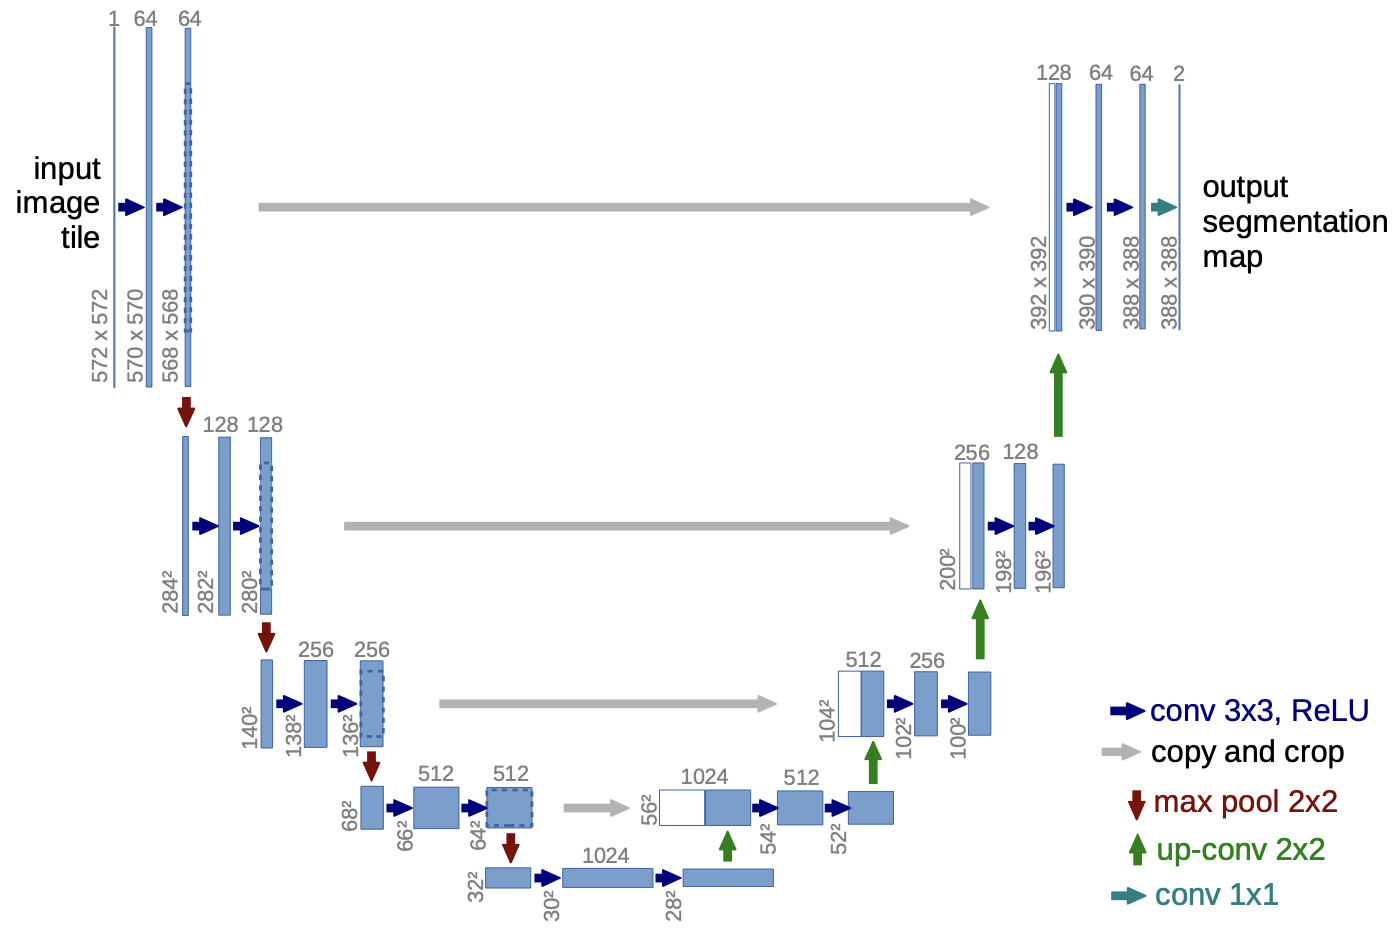
\includegraphics[width=0.5\textwidth]{unet_structure.png}
    \caption{UNet architecture from \cite{unet}.\label{fig:unet}}
\end{figure}
\pagebreak


\subsection{Losses} % Repr. of outputs, how loss is designed to train pose estimation

A combination of Multi-class cross entropy loss and focal loss is used. The Multi-class cross entropy loss is used to regularize pixel-level classification:

\begin{align*}
    L_{\text{entropy}}(x,y)=-\sum_{c=1}^C \log \frac{\exp \left(x_{n, c}\right)}{\sum_{i=1}^C \exp \left(x_{n, i}\right)} y_{n, c}
\end{align*}

where $C=82$ denotes number of classes, subscript $n$ denotes the n-th sample in the batch, $x, y$ denote model 
prediction and ground truth segmentation tensors respectively.

Focal loss is used to address class imbalance issue:

\begin{align*}
    L_{\text {focal }}=&-\alpha\left(1-q_i\right)^\gamma \log \left(q_i\right) \\ & \text { where } q_i=c_i \cdot l_i 
\end{align*}

where $c_i \in \mathbb{R}^C$ is the predicted confidence of the i-th pixel belonging to
each class, and $l_i \in \mathbb{R}^C$ is the ground truth one-hot encoded label of the i-th pixel.

A visualization of segmented output is shown in figure \ref{fig:test_scene}.

\begin{figure}[H]\centering
    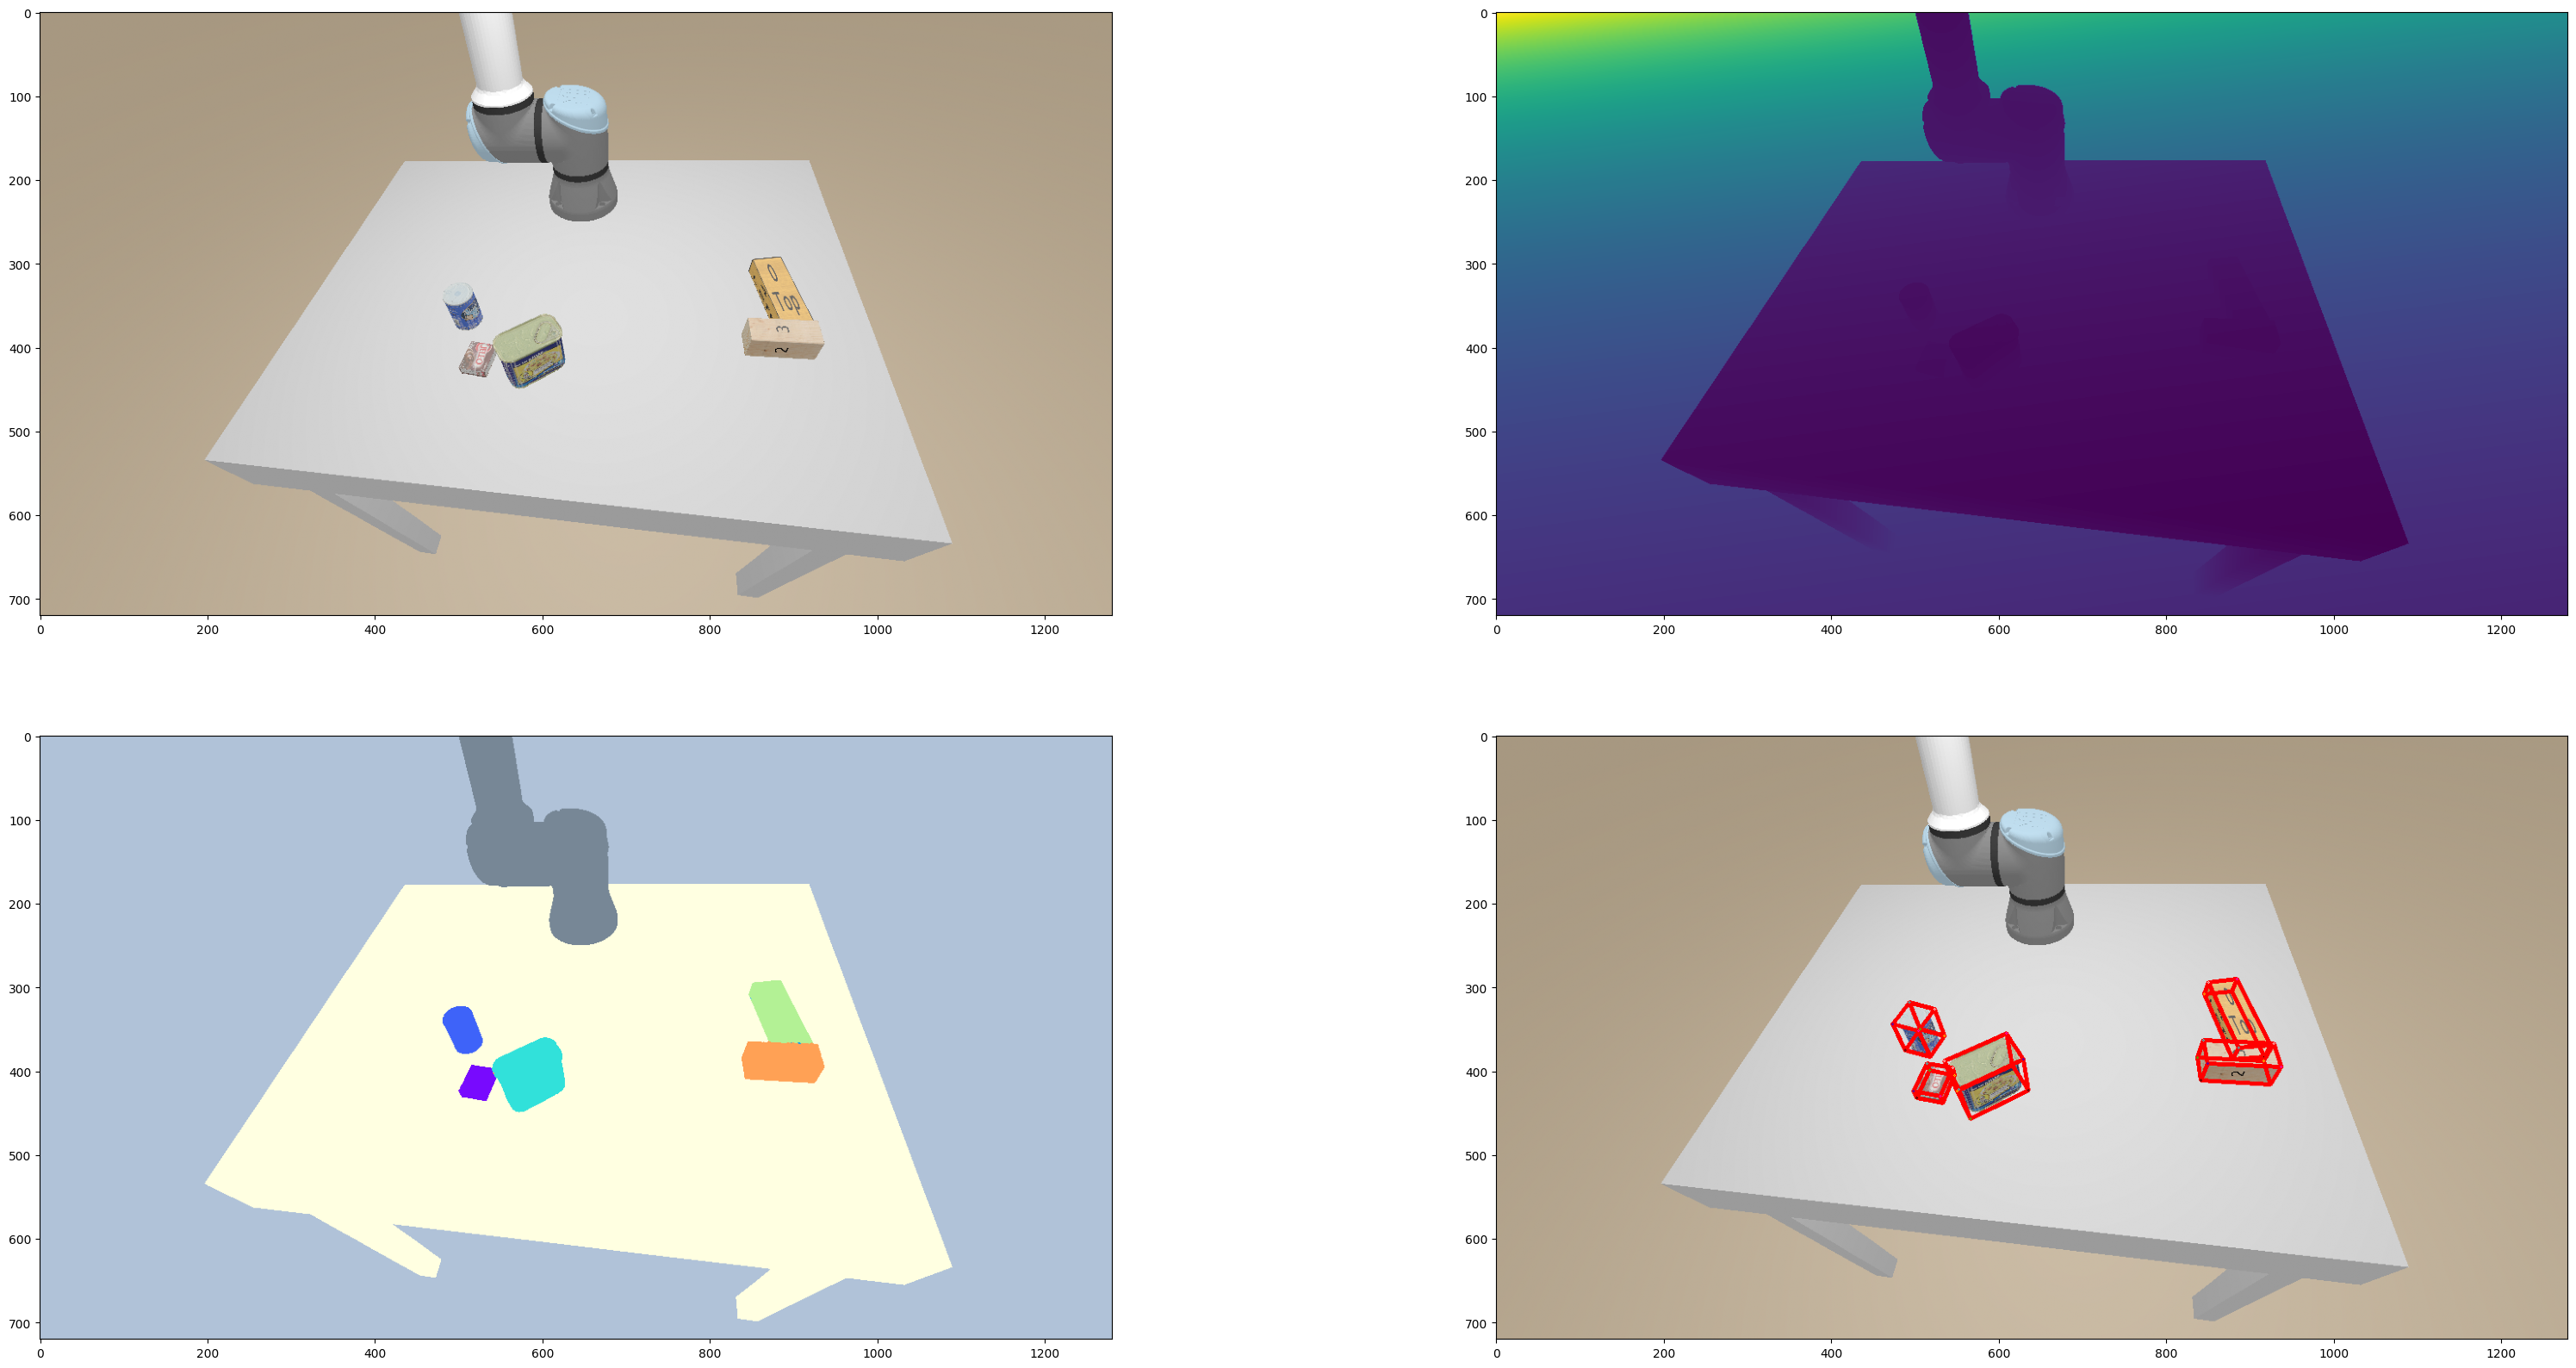
\includegraphics[width=0.7\textwidth]{test_scene.png}
    \caption{Visualization of model output on a test scene. Top left: input RGB
    image. Top right: input depth map. Bottom left: 2D segmentation mask output 
    by UNet. Bottom right: pose estimation. \label{fig:test_scene}}
\end{figure}



\section{Experiments}

\subsection{Data}   % How many data used for training? Pre/post processing

    3964 images with ground truth label are used for training, 236 images
    with ground truth label are used for validation, and 400 images are used for testing.
    No preprocessing is applied. One reason is that the training set has ample images for the UNet to learn a
    good segmentation model (hence no random rotation or horizontal flip are needed
    to increase training set size), another reason is that the original resolution
    image yield better segmentation result than resized images (more details about
    this is discussed in subsection \ref{subsection:ablation}). 

\subsection{Training Details}   % LR, BZ, iters, other hyper-param

    RMSProp algorithm is used to optimize loss function, with learning rate $1e-5$, batch size
    $1$, and 2 epochs. A linear decay learning rate scheduler is alos applied. The batch size was limited to one because of limited GPU memory - 
    only one GPU with 10GB VRAM. 

\subsection{Ablation Studies and Visualization\label{subsection:ablation}}   % Performance of different backbones, BZ, h-param. Runtime analysis w.r.t different design choices.
                                % 1) Performance on validation, 2) failure cases

    First, several different loss function choices are investigated: 1) focal loss only, 
    2) dice loss only (which was adopted by the original UNet paper \cite{unet}), 
    3) cross entropy loss only, 4) cross entropy and focal loss. The segmentation 
    mask output by UNet trained using each of the above loss choices is shown in figure \ref{fig:ablation1}.
    Empirically, the combination of cross entropy and focal losses yield the best result.

    \begin{figure}[H]\centering
        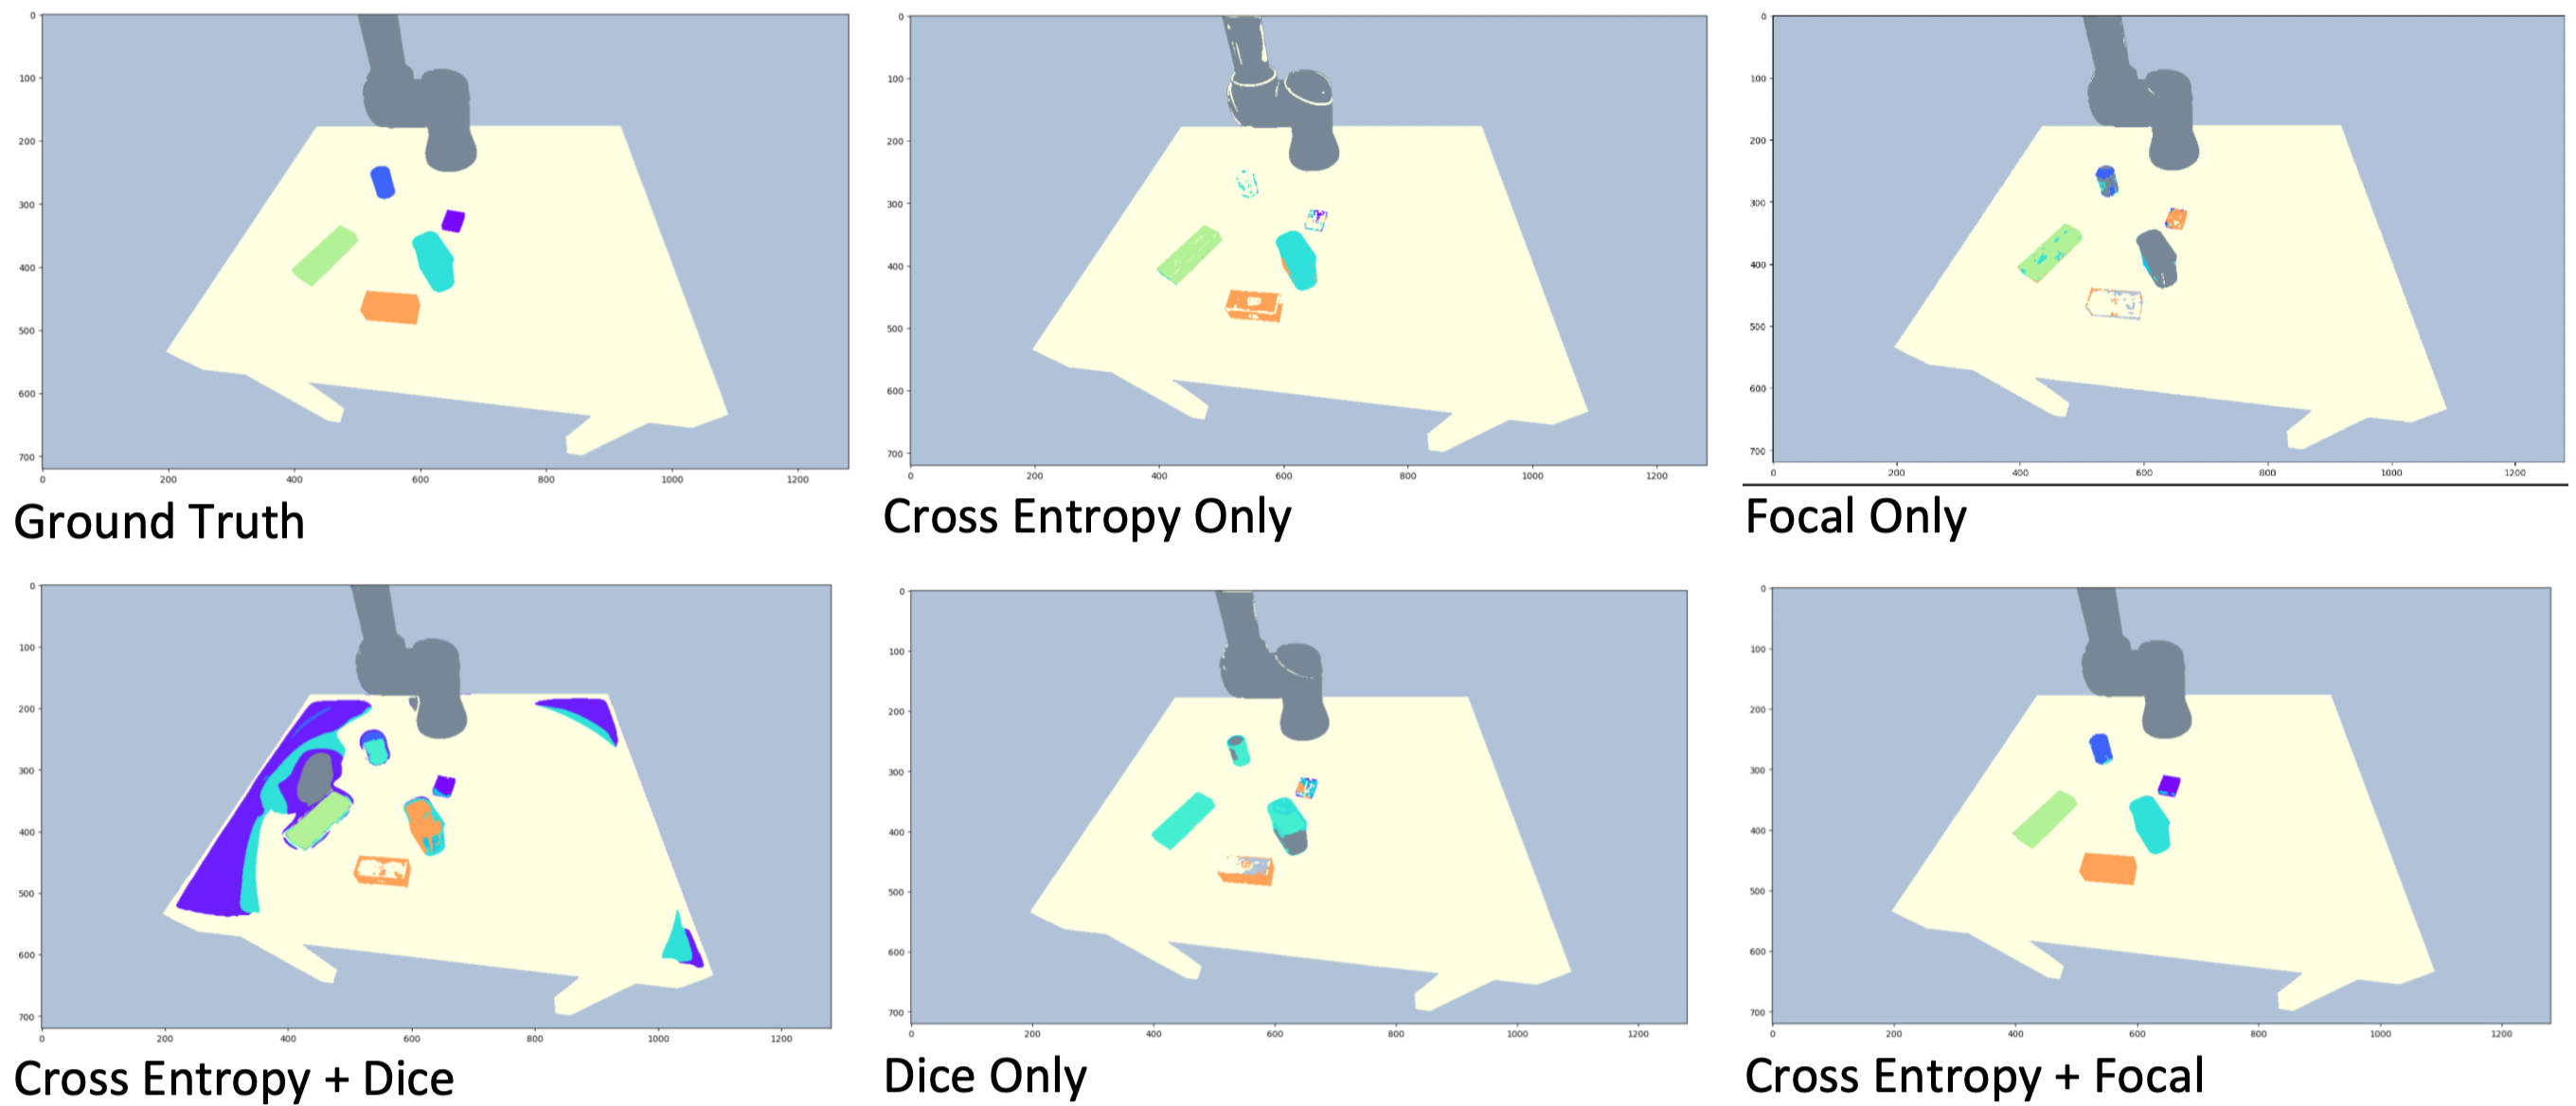
\includegraphics[width=1\textwidth]{ablation1.png}
        \caption{UNet segmentation masks (trained using difference losses).\label{fig:ablation1}}
    \end{figure}
    
    Secondly, the effect of inappropriate learning rate and or over-fitting is investigated
    by adopting an unreasonably large learning rate (i.e. 1e-2) and epochs (i.e. 50), while using
    the optimal loss combination. As shown in figure \ref{fig:ablation2}, overfitting leads
    to a degenerative model that's incapable of producing fine-grained segmentation masks for small objects.

    \begin{figure}[H]\centering
        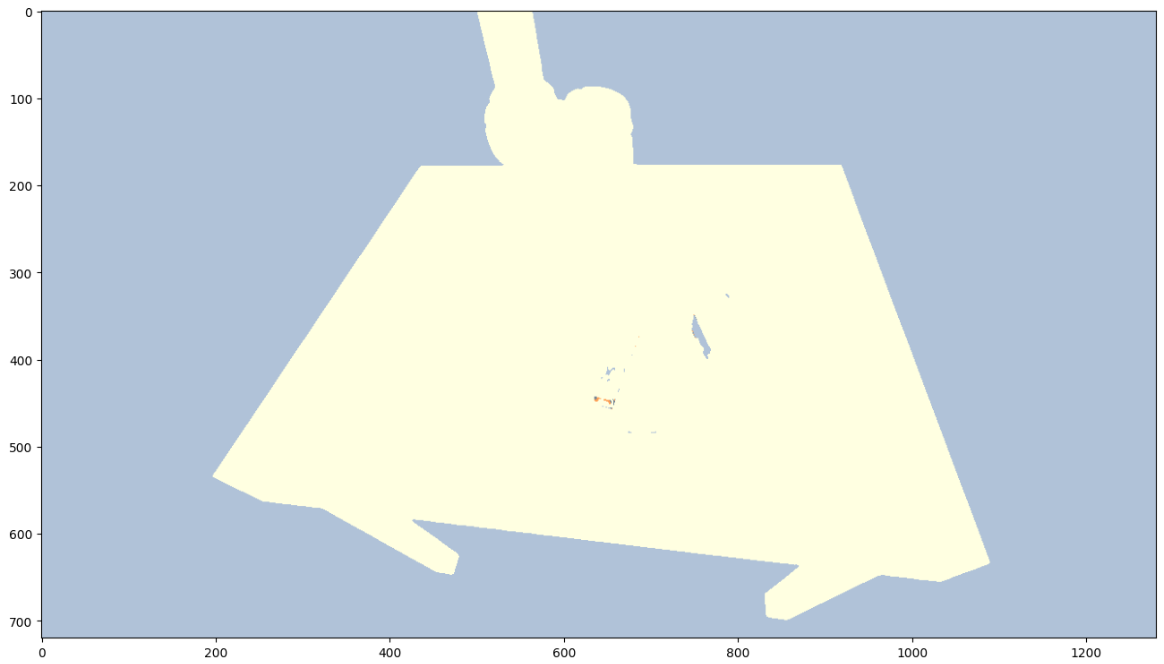
\includegraphics[width=0.5\textwidth]{ablation2.png}
        \caption{Segmentation mask produced by overfitted UNet.\label{fig:ablation2}}
    \end{figure}

    Thirdly, to further justify the loss choice, the effect of segmentation mask quality on pose estimation result 
    is investigated. As shown in figure \ref{fig:ablation3}, a low-quality segmentation mask is sparse 
    for some objects, thereby dramatically reducing the target points available for the IPC algorithm,
    resulting in inferior results.

    \begin{figure}[H]\centering
        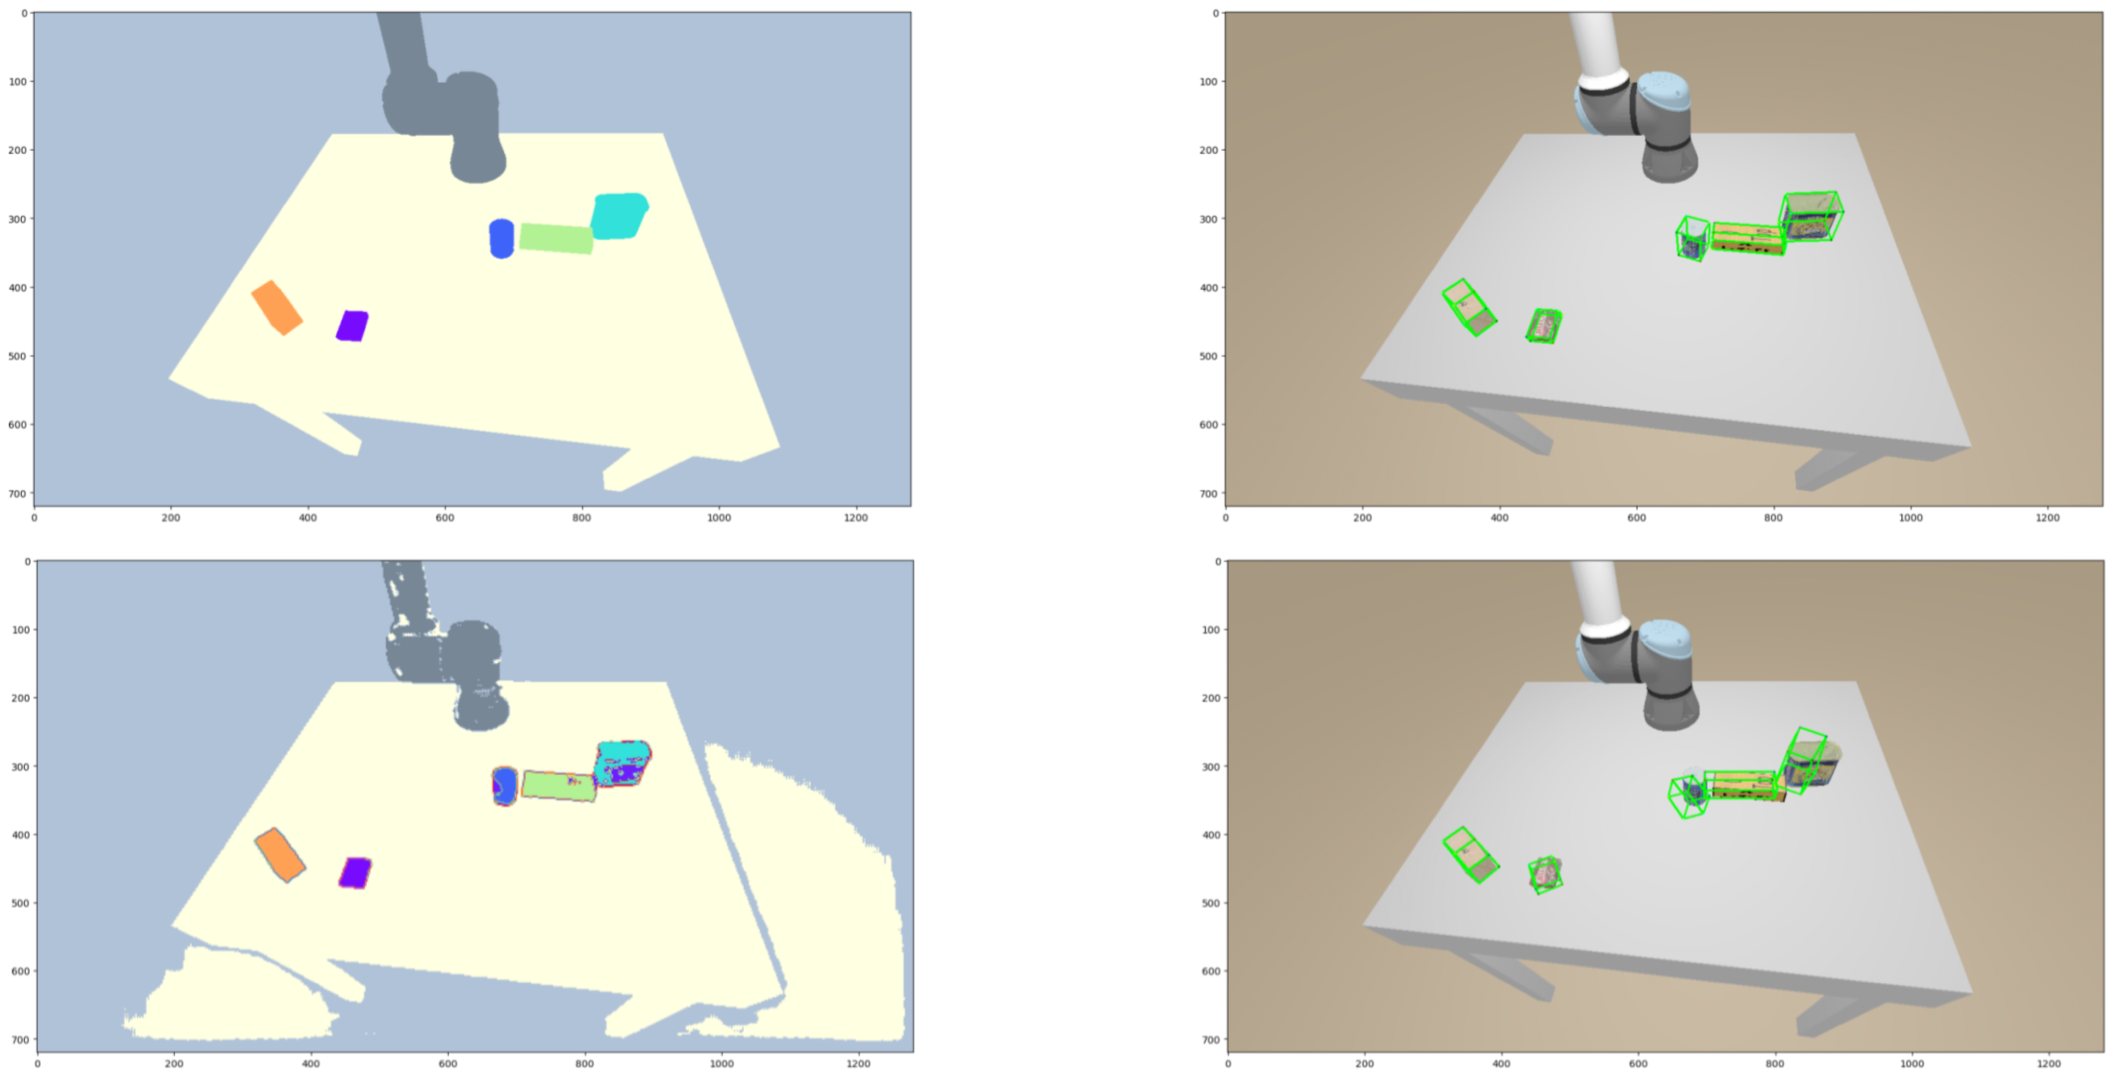
\includegraphics[width=0.8\textwidth]{ablation3.png}
        \caption{Top row: Pose estimation result using a high-quality segmentation mask.
        Bottom row: Pose estimation result using a low-quality segmentation mask.\label{fig:ablation3}}
    \end{figure}
    

\subsection{Performance}    % final performance on benchmark.


The model achieves \textbf{66\%, 71\%} accuracy for 5 degree and 10 degree pose respectively. The submission is available 
through \href{https://storage1.ucsd.edu/cse291ibenchmark/benchmark3}{this link} (user name is \textbf{k5wang}).


\printbibliography

\end{document}